% 图 84.1 —— 由 `checks/emit_hand.py` 自动拼出（probe 精测 + prims2 图元分解）
%%
% ⚠ 这是**稿子不是成品**：跑 `checks/checkhand.py 84.1` 看指标 + 看叠合图。
%%
%% ⚠ 待核：
%   · 本图 probe 报出阴影族 1 个 —— **本脚本不生成阴影**（要照原书手写）；prims2 的 strokes 里可能含阴影线，核对时留意别画重
%   · 可疑字形 1 项（空心圈 ⊙ 常被认成字母 o）—— 见文件末
%%
\documentclass[12pt]{standalone}
\usepackage{fontspec}
\setsansfont{Arial}
\newfontfamily\mfallback{DejaVu Sans}
\usepackage{tikz}
\usetikzlibrary{arrows.meta}
\begin{document}
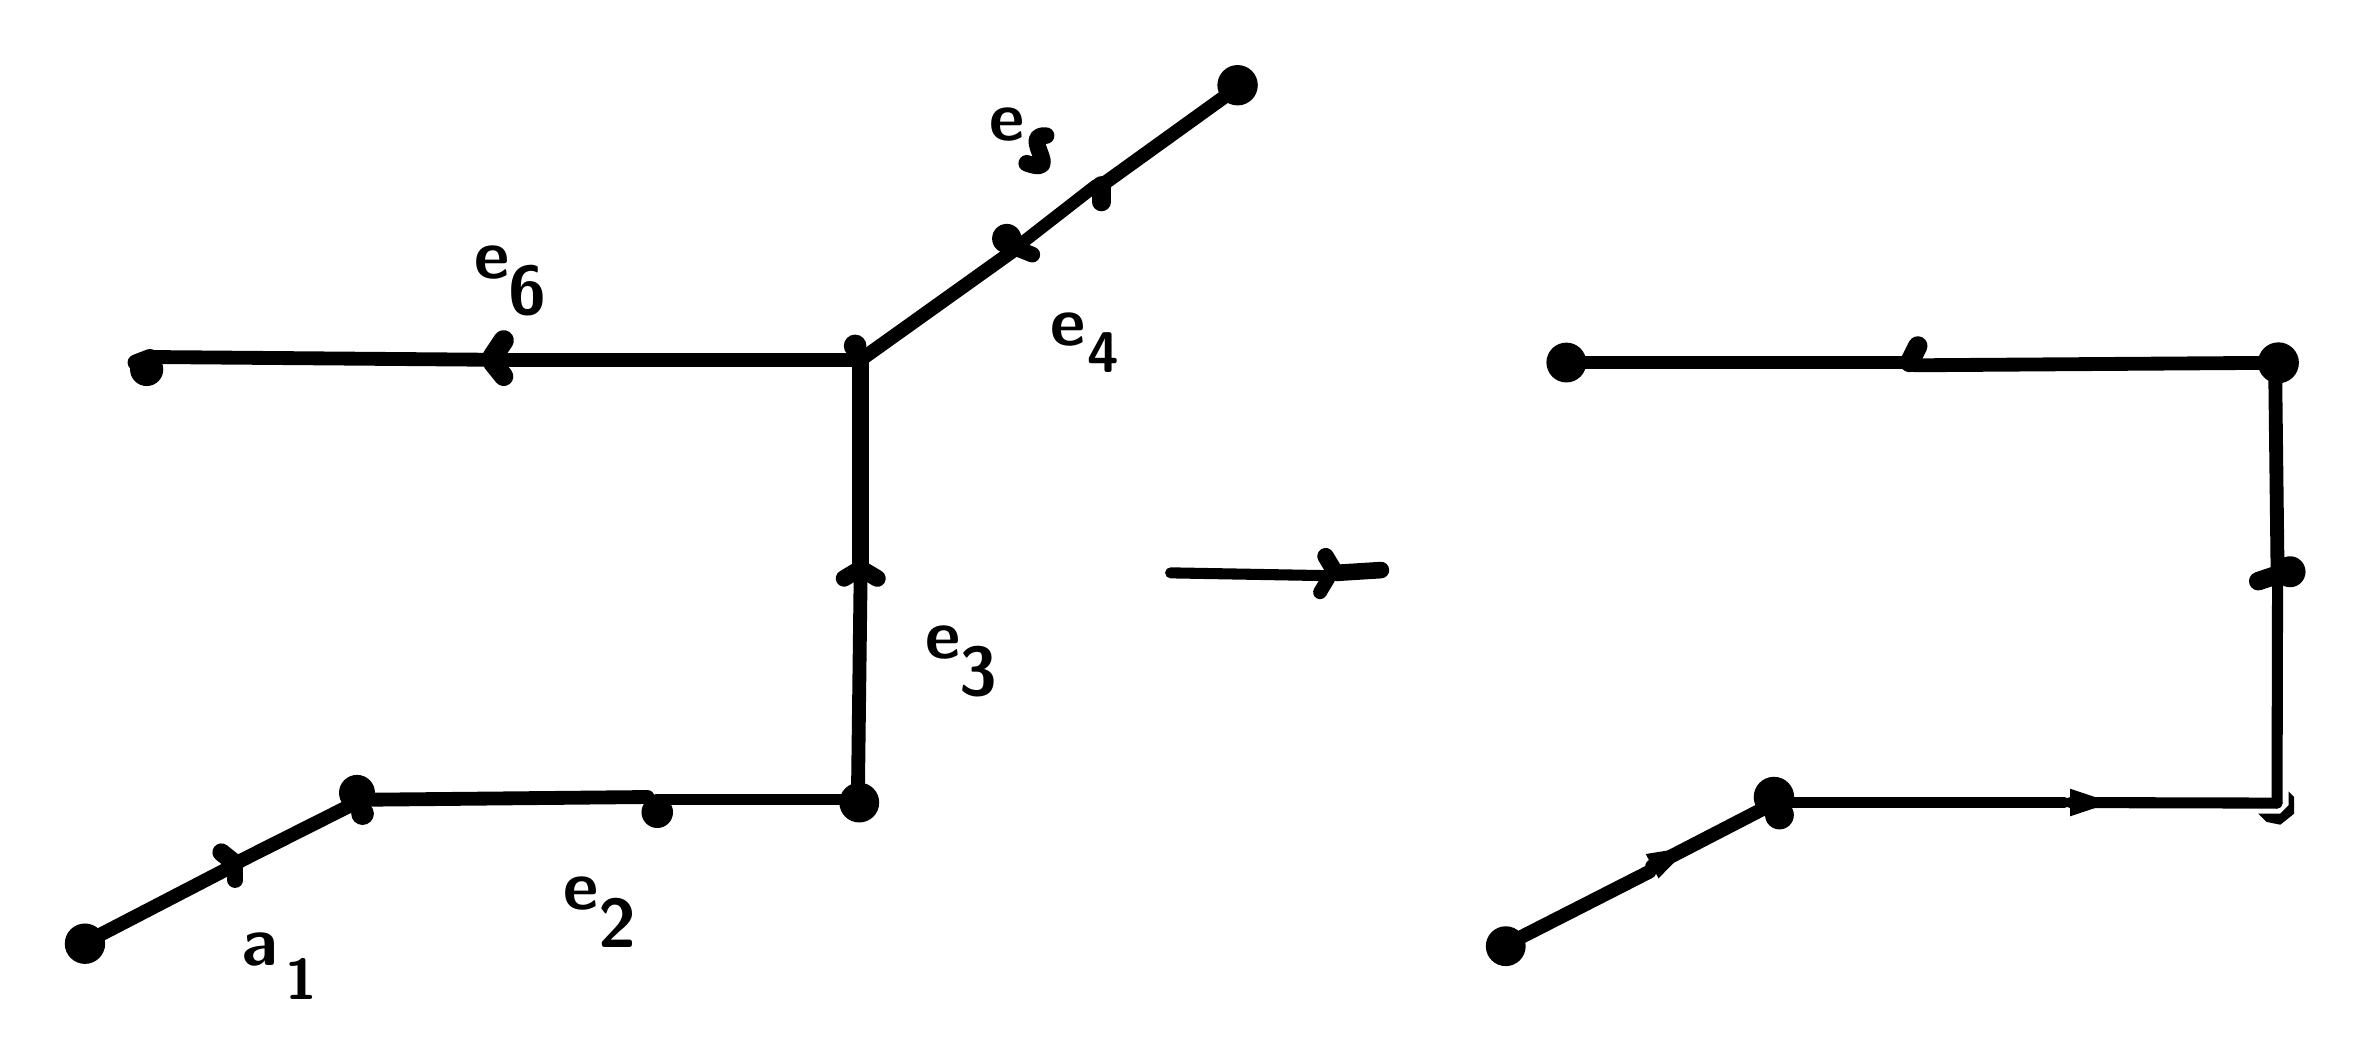
\begin{tikzpicture}[x=1pt, y=-1pt, line width=5.8pt, line cap=round, line join=round]

  %% ════ 填充区（prims2 的 fills）════
  \fill (819.0,278.0) -- (817.0,276.0) -- (817.0,281.0) -- (814.0,284.0) -- (806.0,284.0) -- (809.0,287.0) -- (814.0,288.0) -- (819.0,284.0) -- cycle;

  %% ════ 直线段（prims2 的 strokes）════
  \draw[line width=5.8pt] (39.0,121.0) -- (44.2,119.0);
  \draw[line width=5.0pt] (44.2,119.0) -- (167.0,120.0);
  \draw[line width=7.0pt] (172.0,126.0) -- (168.0,121.0);
  \draw[line width=5.7pt] (358.0,80.0) -- (363.0,82.0);
  \draw[line width=6.7pt] (388.0,63.0) -- (388.0,57.0);
  % （略）线段 (582.0,299.0)-(587.0,303.0) 线宽6.5 —— 是箭头头那一坨，已由箭头头代替
  \draw[line width=7.4pt] (172.0,113.0) -- (168.0,119.0);
  \draw[line width=5.0pt] (533.0,332.0) -- (586.0,305.0);
  \draw[line width=5.7pt] (75.0,308.0) -- (75.0,303.0);
  \draw[line width=5.0pt] (679.0,121.0) -- (557.2,121.0);
  \draw[line width=3.8pt] (557.2,121.0) -- (557.0,118.0);
  \draw[line width=5.0pt] (470.0,199.0) -- (467.0,204.0);
  \draw[line width=4.5pt] (386.0,57.0) -- (359.0,78.0);
  \draw[line width=6.0pt] (301.0,195.0) -- (301.0,121.0);
  \draw[line width=6.0pt] (300.0,196.0) -- (295.0,199.0);
  \draw[line width=7.0pt] (683.0,115.0) -- (680.0,121.0);
  \draw[line width=5.0pt] (388.0,57.0) -- (438.0,21.0);
  \draw[line width=5.0pt] (682.0,122.0) -- (812.1,121.1);
  \draw[line width=5.0pt] (812.1,121.1) -- (813.0,197.0);
  \draw[line width=4.0pt] (738.0,280.0) -- (812.8,280.2);
  \fill (738.0,285.0) -- (738.0,275.0) -- (753.0,280.0) -- cycle;
  \draw[line width=4.0pt] (812.8,280.2) -- (813.0,199.0);
  \draw[line width=6.1pt] (302.0,196.0) -- (307.0,199.0);
  \draw[line width=6.5pt] (75.0,302.0) -- (70.0,298.0);
  \draw[line width=5.0pt] (75.0,302.0) -- (120.7,279.0);
  \draw[line width=5.0pt] (120.7,279.0) -- (224.0,278.0);
  \draw[line width=5.0pt] (74.0,303.0) -- (20.0,331.0);
  \draw[line width=5.0pt] (300.0,120.0) -- (169.0,120.0);
  \draw[line width=5.0pt] (357.0,80.0) -- (301.0,120.0);
  \draw[line width=6.0pt] (489.0,196.0) -- (473.0,197.0);
  \draw[line width=5.0pt] (300.0,278.0) -- (301.0,197.0);
  \draw[line width=4.0pt] (299.0,279.0) -- (227.0,279.0);
  \draw[line width=5.0pt] (587.0,303.0) -- (631.5,280.0);
  \fill (589.3,307.4) -- (584.7,298.6) -- (600.3,296.1) -- cycle;
  \draw[line width=4.0pt] (631.5,280.0) -- (736.0,280.0);
  \draw[line width=6.7pt] (806.0,200.0) -- (812.0,198.0);
  % （略）线段 (734.0,274.0)-(737.0,279.0) 线宽6.1 —— 是箭头头那一坨，已由箭头头代替
  \draw[line width=6.0pt] (472.0,196.0) -- (469.0,191.0);
  \draw[line width=4.0pt] (469.0,198.0) -- (413.0,197.0);

  %% ════ 曲线（prims2 的 curves —— 三段式，坐标同为 (y,x)）════
  \draw[line width=6.0pt] (361.0,49.0) .. controls (374.7,53.9) and (358.1,38.3) .. (368.0,39.0);

  %% ════ 实心点 ════
  \fill (437.2,20.8) circle (7.3);
  \fill (353.8,76.2) circle (5.3);
  \fill (299.0,115.0) circle (4.1);
  \fill (556.0,121.0) circle (7.2);
  \fill (813.3,121.1) circle (7.4);
  \fill (43.0,123.5) circle (6.0);
  \fill (817.5,196.6) circle (5.6);
  \fill (119.0,276.5) circle (6.5);
  \fill (631.0,278.0) circle (7.3);
  \fill (300.5,280.0) circle (7.2);
  \fill (227.5,283.5) circle (5.7);
  \fill (121.0,284.0) circle (4.1);
  \fill (633.0,284.5) circle (5.2);
  \fill (20.7,331.0) circle (7.3);
  \fill (534.1,331.9) circle (7.2);

  %% ════ 标签（probe 直接给的 \node 行）════
  %% ⚠ 全部补了 fill=white：文字在最上层，否则与曲线交叉干扰
     \node[anchor=center,inner sep=0pt,fill=white,font=\fontsize{31.4}{39.3}\selectfont] at (353.8,35.1) {\textsf{\textbf{\textit{e}}}};   % box(344,25,16,17)
     \node[anchor=center,inner sep=0pt,fill=white,font=\fontsize{31.4}{39.3}\selectfont] at (167.8,85.1) {\textsf{\textbf{\textit{e}}}};   % box(158,75,16,17)
     \node[anchor=center,inner sep=0pt,fill=white,font=\fontsize{24.4}{30.5}\selectfont] at (180.6,95.1) {\textsf{\textbf{6}}};   % box(174,86,12,17)
     \node[anchor=center,inner sep=0pt,fill=white,font=\fontsize{31.4}{39.3}\selectfont] at (375.8,109.1) {\textsf{\textbf{\textit{e}}}};   % box(366,99,16,17)
     \node[anchor=center,inner sep=0pt,fill=white,font=\fontsize{22.8}{28.5}\selectfont] at (388.8,117.4) {\textsf{\textbf{4}}};   % box(382,109,12,16)
     \node[anchor=center,inner sep=0pt,fill=white,font=\fontsize{31.4}{39.3}\selectfont] at (330.8,222.1) {\textsf{\textbf{\textit{e}}}};   % box(321,212,16,17)
     \node[anchor=center,inner sep=0pt,fill=white,font=\fontsize{23.3}{29.1}\selectfont] at (343.4,232.6) {\textsf{\textbf{3}}};   % box(337,224,12,16)
     \node[anchor=center,inner sep=0pt,fill=white,font=\fontsize{31.4}{39.3}\selectfont] at (199.8,313.1) {\textsf{\textbf{\textit{e}}}};   % box(190,303,16,17)
     \node[anchor=center,inner sep=0pt,fill=white,font=\fontsize{23.6}{29.6}\selectfont] at (213.1,323.9) {\textsf{\textbf{2}}};   % box(207,315,11,17)
     \node[anchor=center,inner sep=0pt,fill=white,font=\fontsize{32.0}{40.0}\selectfont] at (84.1,333.1) {\textsf{\textbf{\textit{a}}}};   % box(75,323,16,17)
     \node[anchor=center,inner sep=0pt,fill=white,font=\fontsize{21.5}{26.9}\selectfont] at (99.0,343.9) {\textsf{\textbf{1}}};   % box(93,336,7,15)

  % 钉死画布：否则超出的图元/控制点会把页面撑大，1:1 回比就失准
  \pgfresetboundingbox
  \path[use as bounding box] (0,0) rectangle (835,359);
\end{tikzpicture}
\end{document}

% ⚠ 待核清单（probe 拿不准，人眼过一遍）：
%   · 未识别/跳过：⑤ 跳过/未识别的字形
